%------------------------------------------------
\section{Lorem ipsum dolor}
%------------------------------------------------
\subsection{Velit scelerisque in dictum}
%---
\begin{frame}
\frametitle{basics}

\begin{itemize}
    \item<+-|alert@+> Mattis ullamcorper velit sed ullamcorper morbi tincidunt ornare \footfullcite{Schrodinger:1926xyk}
    \begin{equation*}
        \hat H \Psi=i \hbar \frac{\partial}{\partial t}\Psi
    \end{equation*}

    \item<+-|alert@+> Quam viverra orci sagittis eu volutpat odio facilisis mauris
    \begin{equation*}
        - \frac{\hbar^2}{2m}\nabla^2 \Psi(\mathbf{r},t)+V(\mathbf{r},t)\Psi(\mathbf{r},t) =i\hbar\frac{\partial}{\partial t}\Psi(\mathbf{r},t)
    \end{equation*}

    \item<+-|alert@+> Lorem ipsum dolor sit amet
    \begin{itemize}
        \item<+-|alert@+> consectetur adipiscing elit
        \item<+-|alert@+> sed do eiusmod tempor incididunt
        \item<+-|alert@+> Leo vel fringilla est ullamcorper
    \end{itemize}
\end{itemize}


\end{frame}
%---
\begin{frame}
\frametitle{blocks}
    % Blocks styles
    % change to color if you want at beamercolorthemeUSC.sty
    \begin{block}{this is a block}
        this is text inside a block.
    \end{block}

    \begin{alertblock}{this is an alertblock}
        this is text inside an alertblock.
    \end{alertblock}

    \begin{exampleblock}{this is an exampleblock\footnotemark}
        this is text inside an exampleblock.
    \end{exampleblock}

    \footnotetext{this is a footnote}
\end{frame}
%---
\subsection{Suspendisse potenti nullam}
\begin{frame}
\frametitle{multi columns}

\begin{columns}[c]

\begin{column}{.25\textwidth}
\begin{figure}
    \centering
    
\includegraphics[width=\textwidth]{figures/trumpy.jpeg}
    \caption{Lorem ipsum}
\end{figure}
\end{column}


\begin{column}{.25\textwidth}
% only uncover after 4-
\uncover<4->{
\begin{figure}
    \centering
    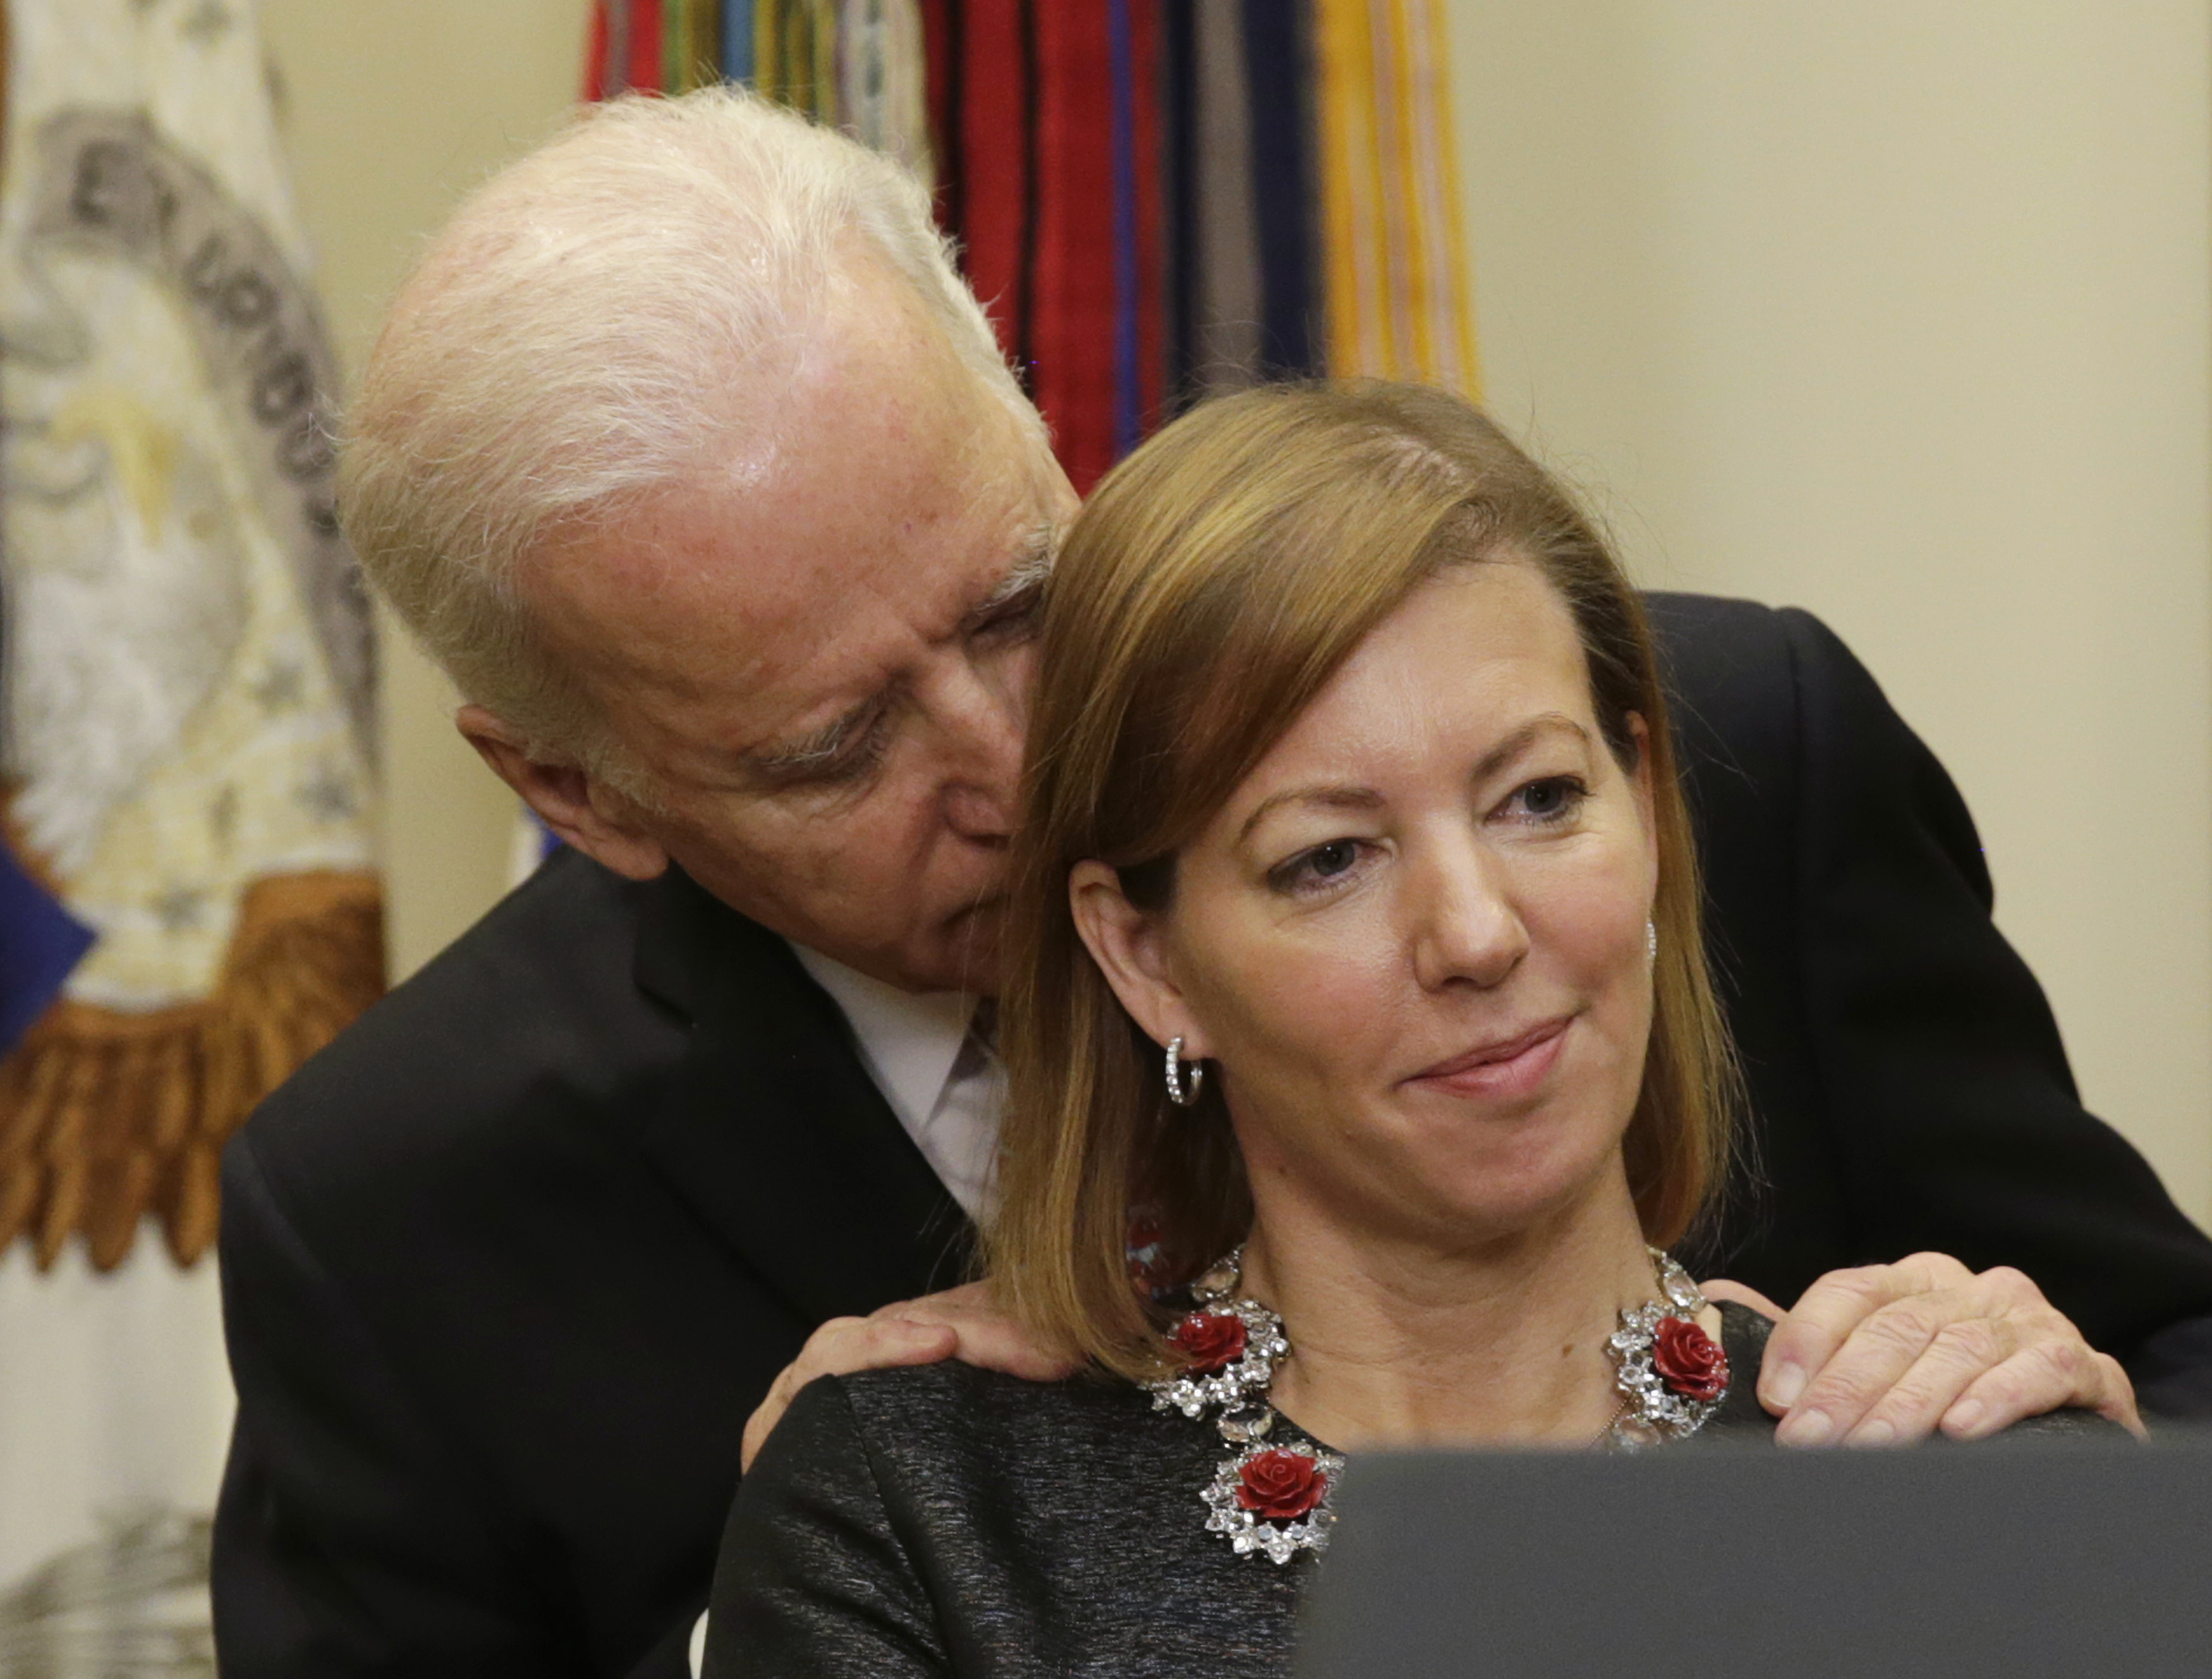
\includegraphics[width=\textwidth]{figures/biddy.jpg}
    \caption{Lorem ipsum}
\end{figure}
}
\end{column}


\begin{column}{.4\textwidth}
\textbf{lorem ipsum:}
\begin{itemize}
    \item<2-|alert@2>  Lorem ipsum dolor sit amet, consectetur adipiscing elit;
    \item<3-|alert@3>  Senectus et netus et malesuada fames ac turpis egestas maecenas
\end{itemize}
\onslide<4->
\textbf{malesuada fames:}
\begin{itemize}
    \item<5-|alert@5> Suspendisse potenti nullam ac tortor vitae purus
    \item<6-|alert@6> A diam sollicitudin tempor id eu
\end{itemize}

\end{column}
\end{columns}


\end{frame}
%---

%------------------------------------------------
\section{Suspendisse potenti nullam}
\begin{frame}
\frametitle{tikz}
\begin{equation*}
    \frac{\partial}{\partial t} \tikzmark{U} \mathbf{U} + \nabla\cdot\tikzmark{F}\mathbf{F} = 0
\end{equation*}

\vspace{15pt}

\begin{equation*}
    \tikzmark{udef}\mathbf{U} = 
    \begin{bmatrix}
        \rho \\
        \rho u \\
        \rho \rho e
    \end{bmatrix}, \quad
    \tikzmark{fdef} \mathbf{F} = 
    \begin{bmatrix}
        \rho u \\
        \rho u^2 + p \\
        \rho e u + p u
    \end{bmatrix}
\end{equation*}

\begin{equation*}
    p = \rho R T\; e = \frac{p}{\gamma - 1} + \frac{1}{2}\rho u^2
\end{equation*}

\begin{tikzpicture}[remember picture, overlay]
    \path[draw=magenta,thick,->] ([shift={(0.05in, -0.05in)}]pic cs:U) to [out=90,in=0,distance=-0.4in] ([shift={(0.0in, 0.05in)}]pic cs:udef);
    \path[draw=magenta,thick,->] ([shift={(0.05in, -0.05in)}]pic cs:F) to [out=90,in=0,distance=-0.4in] ([shift={(0.0in, 0.05in)}]pic cs:fdef);
\end{tikzpicture}
    
\end{frame}

%---
\begin{frame}[fragile]
\frametitle{minted}

\begin{columns}[c]
\begin{column}{.5\textwidth}
\begin{minted}{C++}
template<typename... Ts>
auto sumup(Ts... vals) {
    return (vals + ...);
}

int main(int argc, char* argv[]) {
    std::cout << "1 + 2 + 3 + 4 + 5 = " 
              << sumup(1, 2, 3, 4, 5) 
              << std::endl;
}
\end{minted}
\end{column}

\begin{column}{.4\textwidth}
    \begin{enumerate}
        \item lorem ipsum
        \item Suspendisse potenti nullam
        \item ullamcorper velit sed ullamcorper
    \end{enumerate}
\end{column}
\end{columns}
\end{frame}

%---